\documentclass[a4paper,12pt]{article}
\usepackage[a4paper,margin=2.54cm]{geometry}
\usepackage[slovene]{babel}
\usepackage{graphicx}
\graphicspath{ {./img/} }
\usepackage{hyperref}
\usepackage{fontspec}
\usepackage{titlesec}
\usepackage{eso-pic}
\usepackage{multicol}
\usepackage{amsmath}
\usepackage{enumitem}
\usepackage{tabularx}
\usepackage{array}
\usepackage[absolute,overlay]{textpos} % For absolute positioning
\usepackage[ddmmyyyy]{datetime}
\renewcommand{\dateseparator}{. }

\usepackage{fontspec}
\setmainfont{Roboto} 

\title{Fizika 2 - izpeljave}
\author{insightfulbriyan}

\usepackage{titling}
\renewcommand\maketitlehooka{\null\mbox{}\vfill}
\renewcommand\maketitlehookd{\vfill\null}

\newcolumntype{Y}{>{\centering\arraybackslash}X}

\renewcommand{\arraystretch}{2}

% \setlength{\parindent}{0pt} % Izklop zamika za paragraf
% \setlength{\parskip}{1em} % Presledki med paragrafi

\begin{document}
\pagestyle{empty}

\begin{titlingpage}
    \maketitle
\end{titlingpage}

\section{Valovna enačba}
\subsection{}
Faradejev \ref{eq:faradejev_zakon_diferencialna} in Amperov \ref{eq:amperov_zakon_diferencialna} zakon lahko združimo v valovno enačbo.

\subsection{}
\begin{itemize}[itemsep=-20pt]
    \item $$\vec J = 0$$
    \item $$\vec D = \epsilon_0 \vec E$$
    \item $$\vec B = \mu_0 \vec H$$
    \item $$\vec E = (0, E_y(x, t), E_z(x, t))$$
    \item $$\vec H = (0, H_y(x, t), H_z(x, t))$$
\end{itemize}

\subsection{}
\begin{multline}
    \begin{vmatrix}
        \vec{i}                     & \vec{j}                     & \vec{k}                     \\
        \frac{\partial}{\partial x} & \frac{\partial}{\partial y} & \frac{\partial}{\partial z} \\
        E_x                         & E_y                         & E_z
    \end{vmatrix} = \left( \frac{\partial E_z}{\partial y} - \frac{\partial E_y}{\partial z}, \frac{\partial E_x}{\partial z} - \frac{\partial E_z}{\partial x}, \frac{\partial E_y}{\partial x} - \frac{\partial E_x}{\partial y} \right)
    = \left( 0, -\frac{\partial E_z}{\partial x}, \frac{\partial E_y}{\partial x} \right) = \\
    = -\mu_0 \left( \frac{\partial H_x}{\partial t}, \frac{\partial H_y}{\partial t}, \frac{\partial H_z}{\partial t} \right) = -\mu_0 \left( 0, \frac{\partial H_y}{\partial t}, \frac{\partial H_z}{\partial t} \right)
\end{multline}

\begin{multicols}{2}
    \begin{equation}
        \frac{\partial E_z}{\partial x} = \mu_0 \frac{\partial H_y}{\partial t}
    \end{equation}

    \begin{equation}
        \frac{\partial E_y}{\partial x} = -\mu_0 \frac{\partial H_z}{\partial t}
    \end{equation}
\end{multicols}


\subsection{}
\begin{multline}
    \begin{vmatrix}
        \vec{i}                     & \vec{j}                     & \vec{k}                     \\
        \frac{\partial}{\partial x} & \frac{\partial}{\partial y} & \frac{\partial}{\partial z} \\
        H_x                         & H_y                         & H_z
    \end{vmatrix} = \left( \frac{\partial H_z}{\partial y} - \frac{\partial H_y}{\partial z}, \frac{\partial H_x}{\partial z} - \frac{\partial H_z}{\partial x}, \frac{\partial H_y}{\partial x} - \frac{\partial H_x}{\partial y} \right)
    = \left( 0, -\frac{\partial H_z}{\partial x}, \frac{\partial H_y}{\partial x} \right) = \\
    = \epsilon_0 \left( \frac{\partial H_x}{\partial t}, \frac{\partial H_y}{\partial t}, \frac{\partial H_z}{\partial t} \right) = \epsilon_0 \left( 0, \frac{\partial H_y}{\partial t}, \frac{\partial H_z}{\partial t} \right)
\end{multline}

\begin{multicols}{2}
    \begin{equation}
        \frac{\partial H_z}{\partial x} = -\epsilon_0 \frac{\partial E_y}{\partial t}
    \end{equation}

    \begin{equation}
        \frac{\partial H_y}{\partial x} = \epsilon_0 \frac{\partial E_z}{\partial t}
    \end{equation}
\end{multicols}

\newpage
\subsection{}
\begin{table}[h!]
    \centering
    \begin{tabularx}{\textwidth}{YY}
        $\frac{\partial E_y}{\partial x} = -\mu_0 \frac{\partial H_z}{\partial t}$                  & $\frac{\partial H_z}{\partial x} = -\epsilon_0 \frac{\partial E_y}{\partial t}$                             \\
        $\frac{\partial^2 E_y}{\partial x \partial t} = -\mu_0 \frac{\partial^2 H_z}{\partial t^2}$ & $\frac{\partial^2 H_z}{\partial x^2} \frac{1}{- \epsilon_0} = \frac{\partial^2 E_y}{\partial t \partial x}$ \\
    \end{tabularx}
\end{table}

\subsection{}
\begin{equation}
    \frac{\partial^2 E_y}{\partial x^2} \frac{1}{- \mu_0} = -\epsilon_0 \frac{\partial^2 E_y}{\partial t^2}
\end{equation}


\subsection{}
\begin{equation}
    E_y = E_0 \cos(\omega t - k x); \omega = 2 \pi f, k = \frac{\omega}{c_0}
\end{equation}

\begin{equation}
    \frac{\partial^2 E_y}{\partial x^2} = -k^2 E_y; \frac{\partial^2 E_y}{\partial t^2} = -\omega^2 E_y
\end{equation}

\begin{equation}
    k^2 E_y \frac{1}{- \epsilon_0 \mu_0} =  \omega^2 E_y = \frac{\omega^2}{c_0^2} \frac{1}{- \epsilon_0 \mu_0} E_y
\end{equation}

\subsection{}
\begin{equation}
    \frac{1}{\epsilon_0 \mu_0} = c_0^2
\end{equation}


\newpage

\section{Lomni količnik}
\subsection{}
\begin{align}
    c = \frac{1}{\sqrt{\epsilon_r \epsilon_0 \mu_r \mu_0}}; c_0 = \frac{1}{\sqrt{\epsilon_0\mu_0}} \\
    n = \frac{c}{c_0} = \sqrt{\frac{\epsilon_0\mu_0}{\epsilon_r \epsilon_0 \mu_r \mu_0}} = \frac{1}{\sqrt{\epsilon_r \mu_r}}
\end{align}

\newpage

\section{Lomni zakon} \label{sec:lomni_zakon}
\subsection{}
Minimiziramo čas preleta žarkov od točke A do točke B, ki sta v različnih medijih z različnimi $n$.

\subsection{}
$t(\alpha, \beta)$ ima ekstrem, če je $dt = 0$
\begin{align}
    t  & = t_1 + t_2                                                                                                                        \\
    t  & = \frac{s_1}{c_1} + \frac{s_2}{c_2}                                                                                                \\
    t  & = \frac{h_1}{\cos(\alpha) * c_1} + \frac{h_2}{\cos(\beta) * c_2}                                                                   \\
    dt & = \frac{\partial t}{\partial \alpha} d\alpha + \frac{\partial t}{\partial \beta} d\beta = 0                                        \\
       & \frac{h_1 \sin(\alpha)}{\cos^2(\alpha) * c_1} d\alpha = -\frac{h_2 \sin(\beta)}{\cos^2(\beta) * c_2} d\beta                        \\
       & \frac{d \alpha}{d \beta} = - \frac{h_2}{h_1} \frac{c_1}{c_2} \frac{\sin(\beta)}{\sin(\alpha)} \frac{\cos^2(\alpha)}{\cos^2(\beta)}
\end{align}

\subsection{}
$L$ je razdalja med točkama po $y$ osi, ker je konstantna, je $dL = 0$
\begin{align}
    L = l_1 + l_2 = \frac{h_1}{\tan(\alpha)} + \frac{h_2}{\tan(\beta)}             \\
    dL = \frac{h_1}{\cos^2(\alpha)} d\alpha + \frac{h_2}{\cos^2(\beta)} d\beta = 0 \\
    \frac{h_1}{\cos^2(\alpha)} d\alpha = -\frac{h_2}{\cos^2(\beta)} d\beta         \\
    \frac{d \alpha}{d \beta} = -\frac{h_2}{h_1} \frac{\cos^2(\beta)}{\cos^2(\alpha)}
\end{align}

\subsection{}
\begin{align}
    -\frac{h_2}{h_1} \frac{c_1}{c_2} \frac{\sin(\beta)}{\sin(\alpha)} \frac{\cos^2(\alpha)}{\cos^2(\beta)} = - \frac{h_2}{h_1} \frac{\cos^2(\beta)}{\cos^2(\alpha)} \\
    \Rightarrow \frac{\sin(\beta)}{\sin(\alpha)} = \frac{c_1}{c_2} = \frac{\frac{c_0}{n_1}}{\frac{c_0}{n_2}} = \frac{n_2}{n_1}                                      \\
    \Rightarrow n_1 \sin(\alpha) = n_2 \sin(\beta)
\end{align}

\section{Odbojni zakon} \label{sec:odbojni_zakon}
\begin{align}
    t  & = t_1 + t_2                                                                                         \\
    t  & = \frac{s_1}{c} + \frac{s_2}{c}                                                                     \\
    t  & = \frac{h}{\cos(\alpha) * c} + \frac{h}{\cos(\beta) * c}                                            \\
    dt & = \frac{\partial t}{\partial \alpha} d\alpha + \frac{\partial t}{\partial \beta} d\beta = 0         \\
       & \frac{h \sin(\alpha)}{\cos^2(\alpha) * c} d\alpha = -\frac{h \sin(\beta)}{\cos^2(\beta) * c} d\beta \\
       & \frac{d \alpha}{d \beta} = -\frac{\sin(\beta)}{\sin(\alpha)} \frac{\cos^2(\alpha)}{\cos^2(\beta)}
\end{align}

\subsection{}
$L$ je razdalja med točkama po $y$ osi, ker je konstantna, je $dL = 0$
\begin{align}
    L = l_1 + l_2 = \frac{h}{\tan(\alpha)} + \frac{h}{\tan(\beta)}             \\
    dL = \frac{h}{\cos^2(\alpha)} d\alpha + \frac{h}{\cos^2(\beta)} d\beta = 0 \\
    \frac{h}{\cos^2(\alpha)} d\alpha = -\frac{h}{\cos^2(\beta)} d\beta         \\
    \frac{d \alpha}{d \beta} = -\frac{\cos^2(\beta)}{\cos^2(\alpha)}
\end{align}

\subsection{}
\begin{align}
    -\frac{\sin(\beta)}{\sin(\alpha)} \frac{\cos^2(\alpha)}{\cos^2(\beta)}= -\frac{\cos^2(\beta)}{\cos^2(\alpha)} \\
    \Rightarrow \frac{\sin(\beta)}{\sin(\alpha)} = 1                                                              \\
    \Rightarrow \sin(\alpha) = \sin(\beta)                                                                        \\
    \Rightarrow \alpha = \beta
\end{align}

\section{Mikroskop}\label{sec:mikroskop}
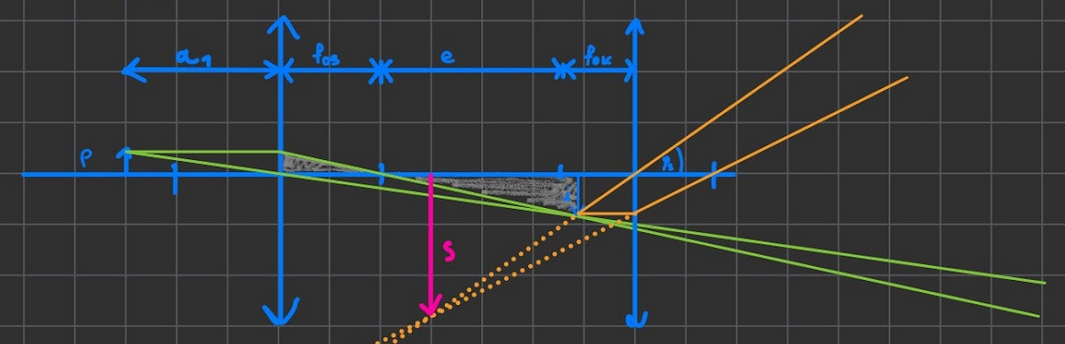
\includegraphics[width=\textwidth]{mikroskop.png}

\begin{align}
    \tan(\varphi_1) = \frac{p}{x_0}             \\
    \tan(\varphi_2) = \frac{i}{f_{ok}}          \\
    \frac{i}{e} = \frac{p}{f_{ob}}              \\
    M = \frac{\tan(\varphi_2)}{\tan(\varphi_1)} \\
    M = \frac{e x_0}{f_{ok} f_{ob}}
\end{align}

\section{Daljnogled}\label{sec:daljnogled}
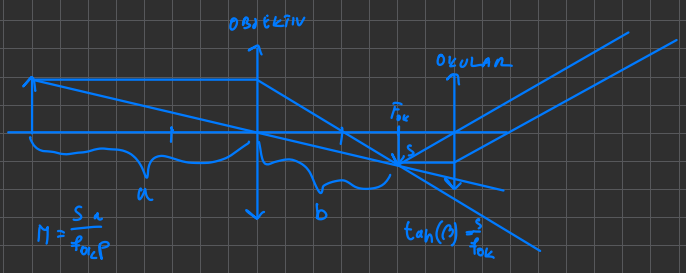
\includegraphics[width=\textwidth]{daljnogled.png}
\begin{align}
    \tan(\varphi_1) = \frac{p}{a} = \frac{s}{b}                                              \\
    \tan(\varphi_2) = \frac{s}{f_{ok}}                                                       \\
    \frac{1}{f_{ob}} = \frac{1}{a} + \frac{1}{b} \Rightarrow b = \frac{a f_{ob}}{a - f_{ob}} \\
    M = \frac{\tan(\varphi_2)}{\tan(\varphi_1)} = \frac{b}{f_{ok}}                           \\
    M = \frac{a f_{ob}}{f_{ok} (a - f_{ob})}
\end{align}

\newpage
\section{Absorpcija EM valovanja}
Telo debeline $x$ in koeficientom absorpcije $\mu$ bo absorbira svetlobni tok $j$.
Tanko telo debeline $dx$ absorbira svetlobni tok $dj$

\begin{align}
    dj                               & = -\mu j dx            \\
    \frac{1}{j} dj                   & = -\mu dx              \\
    \int_{j_0}^{j(x)} \frac{1}{j} dj & = -\mu \int_{0}^{x} dx \\
    \ln(j(x)) - \ln(j_0)             & = -\mu x               \\
    \ln\left(\frac{j(x)}{j_0}\right) & = -\mu x               \\
    j(x)                             & = j_0 e^{-\mu x}
\end{align}

\section{Okrogla luč po Lambertovem zakonu}
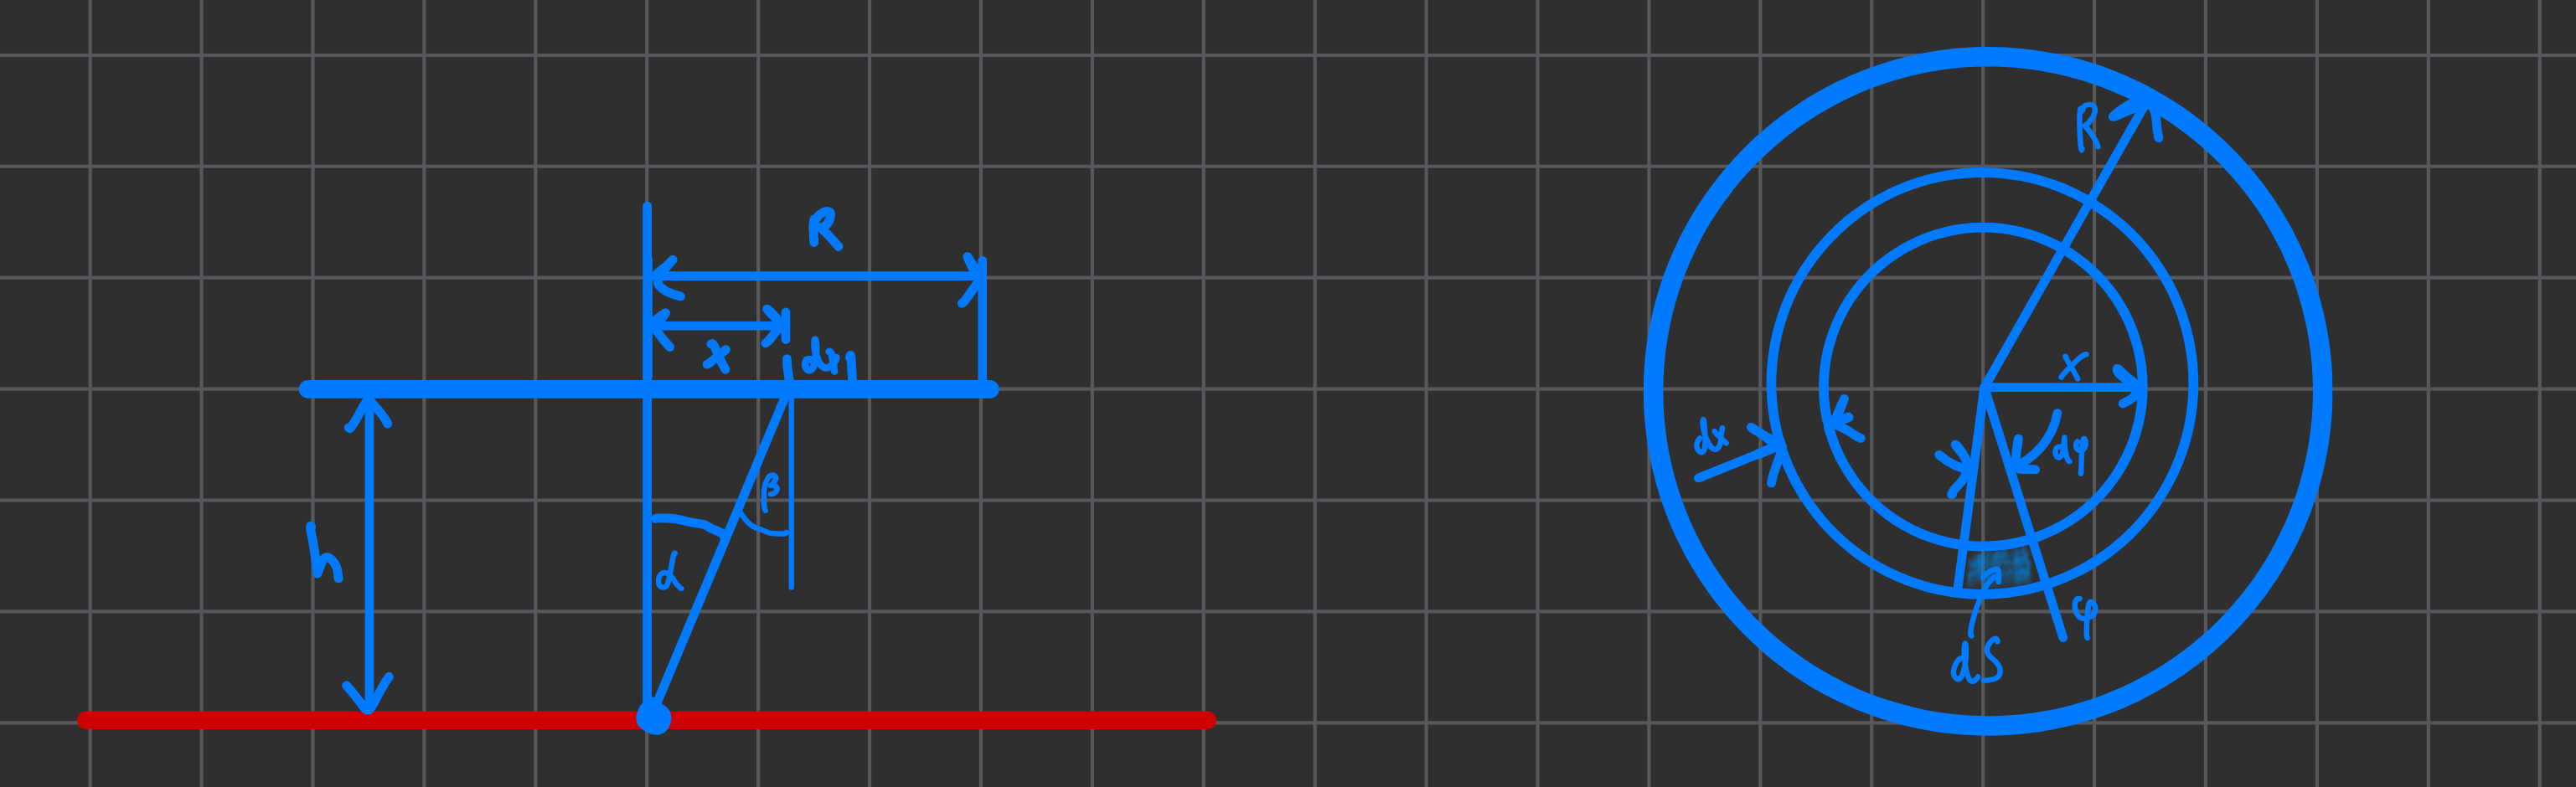
\includegraphics[width=\textwidth]{lambertova_luc.png}
\subsection{}
\begin{align}
    B(\theta) & = B_0                                      \\
    dI        & = B(\theta) \cos(\beta) dS                 \\
    dS        & = x d\varphi dx                            \\
    dS        & = \int_0^{2 \pi} x dx d\varphi             \\
    dS        & = 2 \pi x dx                               \\
    dI        & = B_0 \cos(\beta) 2 \pi x dx               \\
    dE        & = \frac{dI}{r^2} \cos(\beta)               \\
    dE        & = \frac{B_0}{r^2} \cos^2(\beta) 2 \pi x dx
\end{align}

\subsection{}
\begin{align}
    r = \sqrt{x^2 + h^2}                                     \\
    \cos(\beta) = \frac{h}{r}                                \\
    r = \frac{h}{\cos(\beta)}                                \\
    \tan(\beta)  = \frac{x}{h} \Rightarrow x = h \tan{\beta} \\
    \frac{1}{\cos^2(\beta)} d \beta = \frac{1}{h} dx         \\
    dx = h \frac{1}{\cos^2(\beta)} d\beta
\end{align}

\subsection{}
\begin{align}
    \beta(x) & = \arctan\left(\frac{x}{h}\right)           \\
    \beta(0) & = 0                                         \\
    \beta(R) & = \beta_0 = \arctan\left(\frac{R}{h}\right)
\end{align}

\subsection{}
\begin{align}
    E = \int dE = \int_0^{\beta} \frac{B_0 \cos^2(\beta) \cos^2(\beta) 2\pi h \sin(\beta) h}{h^2 \cos(\beta) \cos^2(\beta)} d\beta \\
    E = \int_0^\beta B_0 \sin(\beta) \cos(\beta) 2 \pi d\beta                                                                      \\
    E = B_0 \pi \int_0^{\beta} \sin(2 \beta) d\beta                                                                                \\
    E = B_0 \pi \int_0^{2 \beta} \sin(u) du; u = 2\beta \Rightarrow du = 2 d\beta                                                  \\
    E = \frac{B_0 \pi}{2} (-\cos(u)) \vert_{u=0}^{2\beta}                                                                          \\
    E = \frac{B_0 \pi}{2} (1 - \cos(2\beta))                                                                                       \\
\end{align}

\subsection{}
Če je $R$ velik
\begin{equation}
    \lim_{R \to \infty} E = \lim_{\beta \to \frac{\pi}{2}} \frac{B_0 \pi}{2} (1 - \cos(2\beta_0)) = \frac{B_0 \pi}{2} (1 - \cos(\pi)) = \frac{B_0 \pi}{2} (1 + 1) = B_0 \pi
\end{equation}


\section{Michelson-Morleyev interferometer}
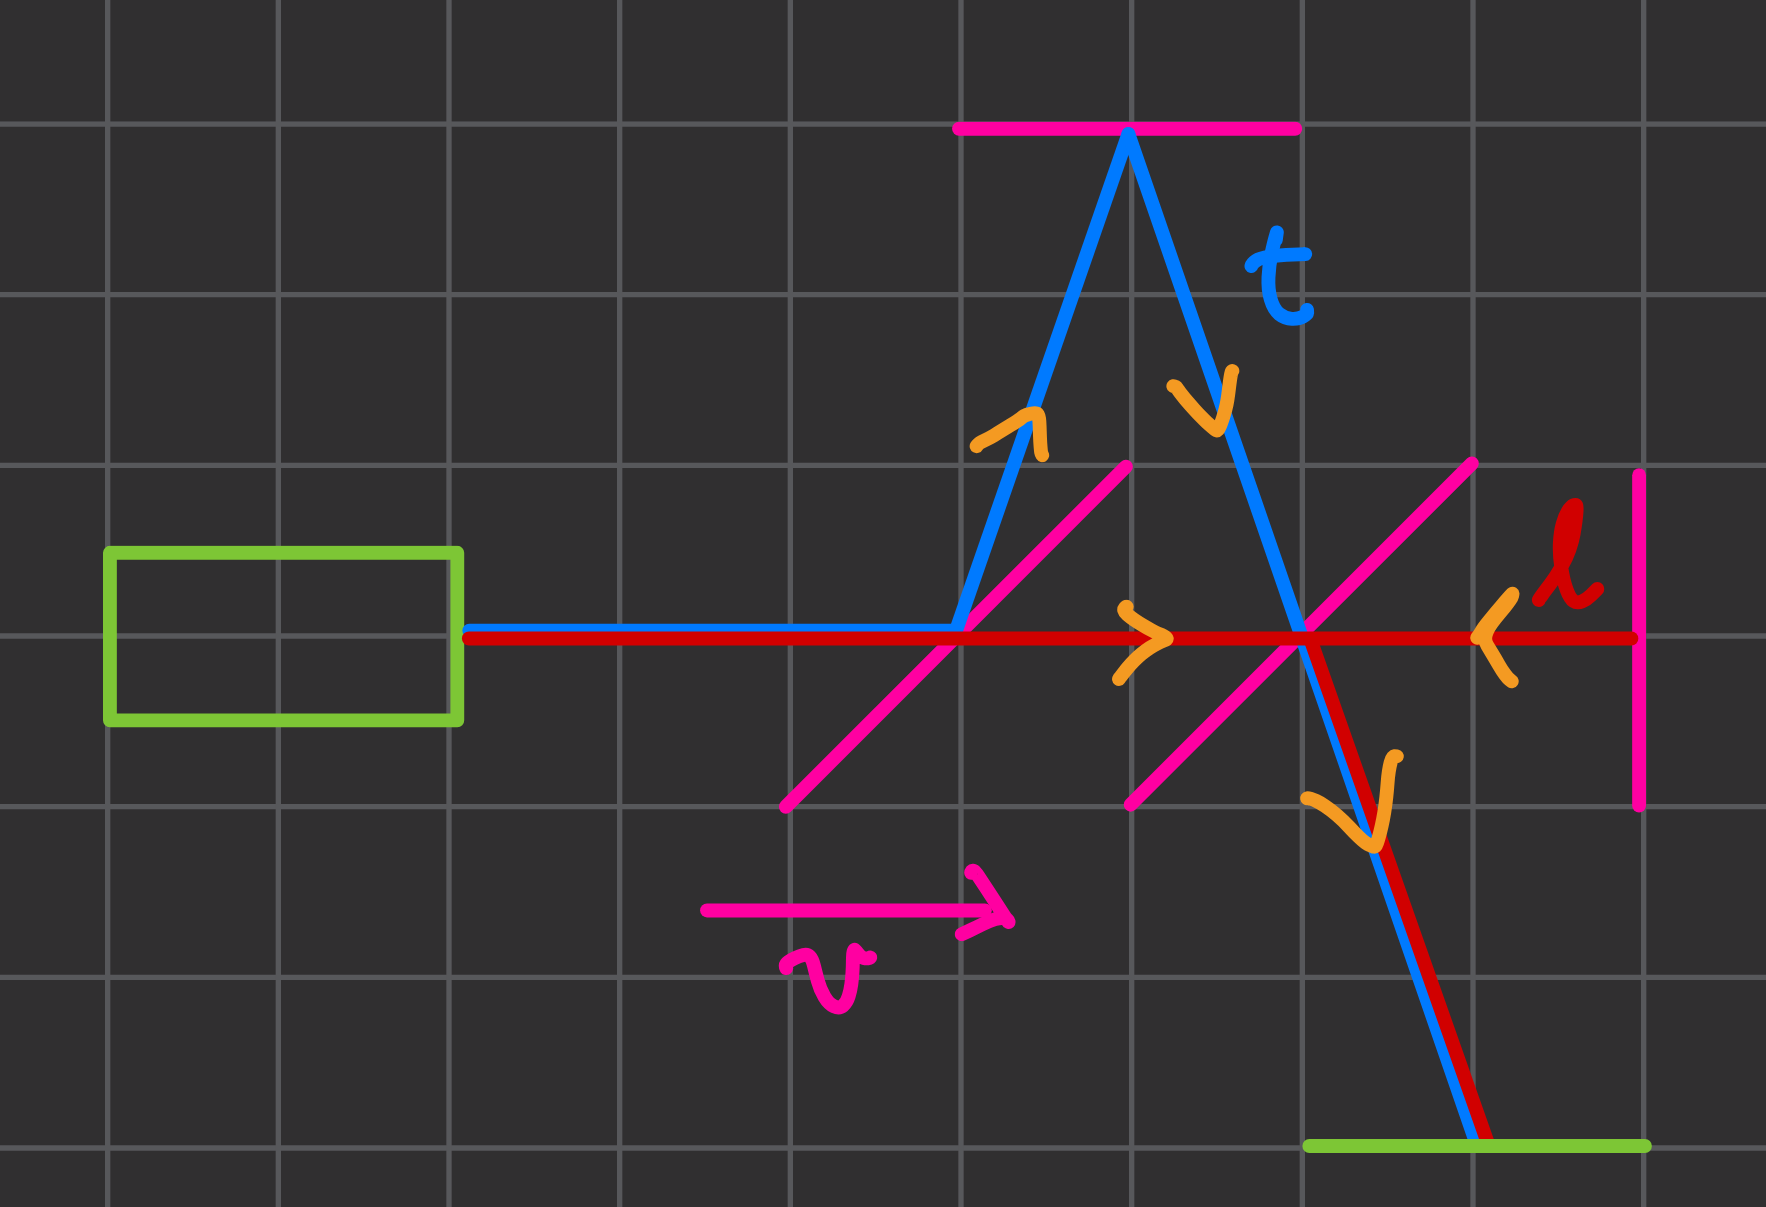
\includegraphics[width=\textwidth]{michelson.png}
\subsection{}
\begin{table}[h!]
    \centering
    \begin{tabularx}{\textwidth}{YY}
        $T_t = \frac{2L}{\sqrt{c^2 - v^2}}$                       & $T_l = \frac{L}{c-v} + \frac{L}{c+v} = \frac{L(c+v) + L(c-v)}{(c-v)(c+v)}$ \\
        $T_t = \frac{2L}{\sqrt{c^2 (1 - \frac{v^2}{c^2})}}$       & $T_l = \frac{2L c}{c^2 - v^2}$                                             \\
        $T_t = \frac{2L}{c} \frac{1}{\sqrt{1 - \frac{v^2}{c^2}}}$ & $T_l = \frac{2L}{c} \frac{1}{1- \frac{v^2}{c^2}}$                          \\
    \end{tabularx}
\end{table}

\subsection{}
\begin{align}
    T_l - T_t & = \frac{2L}{c} \left( \frac{1}{1 - \frac{v^2}{c^2}} - \frac{1}{\sqrt{1 - \frac{v^2}{c^2}}} \right) \\
    (T_l - T_t) c = k \lambda & = 2L \left( (1 + \frac{v^2}{c^2}) - (1 + \frac 1 2 \frac{v^2}{c^2}) \right) \\
    k \lambda & = 2L \frac{1}{2} \frac{v^2}{c^2} = L \frac{v^2}{c^2}
\end{align}

\subsection{}
Če interferometer zavrtimo za 90° lahko zapišemo $k \lambda = -L \frac{v^2}{c^2}$ 
\begin{align}
    n = \frac{k_1\lambda - k_2\lambda}{\lambda} = \frac{L \frac{v^2}{c^2} + L \frac{v^2}{c^2}}{\lambda} = \frac{2 L}{\lambda} \frac{v^2}{c^2}\\
\end{align}

Žal se teoretični izračun ne ujema z eksperimentom

\subsection{}
Če upoštevamo Lorentzovo transformacijo \ref{eq:lorentzova_transformacija} lahko zapišemo
\begin{equation}
    T_l = \frac{2L\sqrt{1 - \frac{v^2}{c^2}}}{c} \frac{1}{1 - \frac{v^2}{c^2}} = \frac{2L}{c} \frac{1}{\sqrt{1 - \frac{v^2}{c^2}}} = T_t
\end{equation}

\section{Stefanov zakon}
Lahko ga izpeljemo z integriranjem Planckovega zakona \ref{eq:planckov_zakon}
\begin{equation}
    j = \int_0^\infty \frac{dj}{d\lambda} d\lambda = \int_0^\infty \frac{2 \pi hc_0^2}{\lambda^5\left(e^{\frac{hc_0}{\lambda k_B T}} - 1\right)} d\lambda
\end{equation}

\subsection{}
$x = \frac{hc_0}{\lambda k_B T} \Rightarrow d\lambda = -\frac{hc_0}{k_B T x^2} dx$ in $\lambda  \to 0 \Rightarrow x \to \infty, \lambda \to \infty \Rightarrow x \to 0$
\begin{align}
    j &= \int_\infty^0 \frac{2 \pi hc_0^2}{\left(\frac{hc_0}{k_B T x}\right)^5 \left(e^x - 1\right)} \left(-\frac{hc_0}{k_B T x^2}\right) dx \\
    j &= \frac{2 \pi (k_B T)^4}{h^3 c_0^3} \int_0^\infty \frac{x^3}{e^x - 1} dx \\
    j &= \frac{2 \pi (k_B T)^4}{h^3 c_0^3} \cdot \frac{\pi^4}{15} = \frac{2 \pi^5 k_B^4 T^4}{15 h^3 c_0^3} \\
    j &= \sigma T^4; \sigma = \frac{2 \pi^5 k_B^4}{15 h^3 c_0^3} = 5,67 \cdot 10^{-8} \frac{\text{W}}{\text{m}^2 \text{K}^4}
\end{align}

\section{Wienov zakon}
Lahko ga izpeljemo z odvajanjem Planckovega zakona \ref{eq:planckov_zakon}
\begin{align}
    \frac{dj}{d\lambda} = \frac{2 \pi hc_0^2}{\lambda^5\left(e^{\frac{hc_0}{\lambda k_B T}} - 1\right)} \\
    \frac{dj}{dx}= \frac{2 \pi k_B^5 T^5}{h^4 c_0^3} \frac{x^5}{e^x - 1}; x = \frac{hc_0}{\lambda k_B T}
\end{align}

\subsection{}
\begin{align}
    \frac{dj}{dx} = A \frac{x^5}{e^x - 1} = 0 \\
    \frac{5x^4 (e^x - 1) - x^5 e^x}{(e^x - 1)^2} = 0 \\
    5x^4 (e^x - 1) - x^5 e^x = 0 \\
    5(e^x - 1) = x e^x \\
    5 = x \frac{e^x}{e^x - 1} \\
    x \approx 4.9651\\
\end{align}

\subsection{}
\begin{align}
    \lambda_{max} = \frac{hc_0}{k_B T x} = \frac{hc_0}{4.9651 k_B T} \\
    \lambda_{max} T = k_W = 2.898 \cdot 10^{-3} \text{m K}
\end{align}


\newpage
\section{Uporabljene enačbe}
\subsection{Matematika}
\begin{multicols}{2}

    \paragraph{Gradient}
    \begin{equation}
        \label{eq:gradient}
        \vec{\nabla} f = \left( \frac{\partial f}{\partial x}, \frac{\partial f}{\partial y}, \frac{\partial f}{\partial z} \right)
    \end{equation}

    \paragraph{Divergenca}
    \begin{equation}
        \label{eq:divergenca}
        \vec{\nabla} \cdot \vec{F} = \frac{\partial F_x}{\partial x} + \frac{\partial F_y}{\partial y} + \frac{\partial F_z}{\partial z}
    \end{equation}

    \paragraph{Rotacija}
    \begin{equation}
        \label{eq:rotacija}
        \vec{\nabla} \times \vec{F} = \begin{vmatrix}
            \vec{i}                     & \vec{j}                     & \vec{k}                     \\
            \frac{\partial}{\partial x} & \frac{\partial}{\partial y} & \frac{\partial}{\partial z} \\
            F_x                         & F_y                         & F_z
        \end{vmatrix}
    \end{equation}

\end{multicols}

\subsection{Maxwellove enačbe}
\begin{multicols}{2}
    \paragraph{Faradejev zakon v integralni obliki}
    \begin{equation}
        \label{eq:faradejev_zakon_integralna}
        \oint \vec{E} \cdot d\vec{l} = -\frac{\partial}{\partial t} \int \vec{B} \cdot d\vec{S}
    \end{equation}

    \paragraph{Faradejev zakon v diferencialni obliki}
    \begin{equation}
        \label{eq:faradejev_zakon_diferencialna}
        \vec{\nabla} \times \vec{E} = -\frac{\partial \vec{B}}{\partial t}
    \end{equation}

    \paragraph{Amperov zakon v integralni obliki}
    \begin{equation}
        \label{eq:amperov_zakon_integralna}
        \int \vec{H} \cdot d\vec{s} = \int J d\vec{S} + \int \frac{\partial \vec{D}}{\partial t} \cdot d\vec{S}
    \end{equation}

    \paragraph{Amperov zakon v diferencialni obliki}
    \begin{equation}
        \label{eq:amperov_zakon_diferencialna}
        \vec{\nabla} \times \vec{H} = \vec{J} + \frac{\partial \vec{D}}{\partial t}
    \end{equation}

\end{multicols}

\subsection{Optika}
\begin{multicols}{2}
    \paragraph{Enačba preslikave}
    \begin{equation}
        \frac{1}{f} = \frac{1}{a} + \frac{1}{b}
    \end{equation}

    \paragraph{Enačba leče}
    \begin{equation}
        \frac{1}{f} = (\frac{n_2}{n_1} - 1) ( \frac{1}{R_1} + \frac{1}{R_2} );
    \end{equation}
    $R > 0$, če je središče krivulje na nasprotni strani leče, kot površina, ki jo opisuje

    \paragraph{Skupek leč}
    \begin{equation}
        \frac{1}{f} = \frac{1}{f_1} + \frac{1}{f_2} - \frac{d}{f_1f_2}
    \end{equation}

    \paragraph{Lomni zakon (\ref{sec:lomni_zakon})}
    \begin{equation}
        n_1 \sin(\alpha) = n_2 \sin(\beta)
    \end{equation}

    \paragraph{Mikroskop (\ref{sec:mikroskop})}
    \begin{equation}
        M = \frac{e x_0}{f_{ok} f_{ob}}
    \end{equation}

    \paragraph{Daljnogled (\ref{sec:daljnogled})}
    \begin{equation}
        M = \frac{a f_{ob}}{f_{ok} (a - f_{ob})}
    \end{equation}
\end{multicols}

\subsection{Moderna fizika}
\begin{multicols}{2}
    \paragraph{Lorentzova transformacija} \label{eq:lorentzova_transformacija}
    \begin{align}
        x' = \gamma (x - vt)              & \qquad x = \gamma (x' + vt')              \\
        y' = y                            & \qquad y = y'                             \\
        z' = z                            & \qquad z = z'                             \\
        t' = \gamma (t - \frac{v}{c^2} x) & \qquad t = \gamma (t' + \frac{v}{c^2} x')
    \end{align}

    \paragraph{Lorentzov faktor}
    \begin{equation}
        \gamma = \frac{1}{\sqrt{1 - \frac{v^2}{c^2}}}
    \end{equation}

    \paragraph{Galilejeva transformacija}
    \begin{align}
        x' = x - vt & \qquad x = x' + vt' \\
        y' = y      & \qquad y = y'       \\
        z' = z      & \qquad z = z'       \\
        t' = t      & \qquad t = t'
    \end{align}

    \paragraph{Planckov zakon} \label{eq:planckov_zakon}
    \begin{equation}
        \frac{dj}{d\lambda} = \frac{2 \pi hc^2}{\lambda^5\left(e^{\frac{hc}{\lambda k_B T}} - 1\right)}
    \end{equation}
\end{multicols}


\end{document}